\documentclass{article}
\usepackage[utf8]{inputenc}
\usepackage[margin=0.75in]{geometry}
\usepackage{enumerate}
\usepackage{amsmath}
\usepackage{amsfonts} 
\usepackage{amssymb}
\usepackage{amsthm}
\usepackage{mathtools}
\usepackage{float}
\usepackage{array}
\usepackage{makecell}
\usepackage{commath}
\usepackage{verbatim}

\DeclarePairedDelimiter{\ceil}{\lceil}{\rceil}

\renewcommand\theadalign{bc}
\renewcommand\theadfont{\bfseries}
\renewcommand\theadgape{\Gape[4pt]}
\renewcommand\cellgape{\Gape[4pt]}

\newcommand{\N}{\mathbb{N}}
\newcommand{\Z}{\mathbb{Z}}
\newcommand{\Q}{\mathbb{Q}}
\newcommand{\C}{\mathbb{C}}
\newcommand{\R}{\mathbb{R}}
\newcommand{\F}{\mathbb{F}}
\newtheorem{theorem}{Theorem}
\newtheorem{corollary}{Corollary}[theorem]
\newtheorem{definition}{Definition}[theorem]
\newtheorem{lemma}[theorem]{Lemma}
\newtheorem*{remark}{Remark}
\newcommand{\cdotscalar}{\;\widetilde{\cdot}\;}
\newcommand{\vectorplus}{\;\widetilde{+}\;}
\newcommand{\Span}{\text{Span}}
\newcommand{\Null}{\text{Null}}
\newcommand{\Range}{\text{Range}}
\newcommand{\D}{\frac{d}{\dif x}}

\renewcommand{\epsilon}{\varepsilon}
\renewcommand{\phi}{\varphi}

\newcommand{\Or}{\mbox{ OR }}
\renewcommand{\And}{\mbox{ AND }}
\newcommand{\Not}{\mbox{NOT }}
\newcommand{\Iff}{\mbox{ IFF }}

\newcommand{\Width}{\textup{width}}
\newcommand{\Mesh}{\textup{mesh}}
\newcommand{\Int}{\textup{Int}}
\newcommand{\Ext}{\textup{Ext}}
\newcommand{\Bd}{\textup{Bd}}
\newcommand{\argmax}{\textup{argmax}}


\newcommand\widebar[1]{\mathop{\overline{#1}}}
\newcommand*\closure[1]{\widebar{#1}}

\newcommand\Ball[2]{U(#1; #2)}

\title{CSC311 Final Project Report}
\author{Anudev Gill and Vishnu Nitoor}
\date{\today}

\begin{document}

\maketitle

\section{}

\begin{enumerate}[(a)]
    \item First, we'll derive the log likelihood $\log(p(C | \theta, \beta))$ for all students and questions. 
    
    We have that 

    \[p(C_{ij} | \theta_i, \beta_j) = p(C_{ij} = 1 | \theta_i, \beta_j)^{C_{ij}} (1 - p(C_{ij} = 1 | \theta_i, \beta_j))^{1 - C_{ij}}\]

    and so 

    \[\log(p(C_{ij} | \theta_i, \beta_j)) = C_{ij} \log(p(C_{ij} = 1 | \theta_i, \beta_j)) + (1 - C_{ij}) \log(1 - p(C_{ij} = 1 | \theta_i, \beta_j))\]

    \begin{align*}
        p(C | \theta, \beta) &= \prod_{i, j} p(C_{ij} | \theta, \beta) \\[1em]
        \log(p(C | \theta, \beta)) &= \sum_{i, j} \log (p(C_{ij} | \theta, \beta)) \\
        &= \sum_{i, j} C_{ij} \log(p(C_{ij} = 1 | \theta_i, \beta_j)) + (1 - C_{ij}) \log(1 - p(C_{ij} = 1 | \theta_i, \beta_j))
    \end{align*}

    Now taking the derivative with respect to $\theta_i$, we have 

    \begin{align*}
        \frac{\partial  \log(p(C | \theta, \beta))}{\partial \theta_i} &= \sum_{j} \frac{\partial}{\partial \theta_i} \left(C_{ij} \log(p(C_{ij} = 1 | \theta_i, \beta_j)) + (1 - C_{ij}) \log(1 - p(C_{ij} = 1 | \theta_i, \beta_j))\right) \\
        &= \sum_{j} C_{ij} \cdot \frac{1}{\sigma(\theta_i - \beta_j)} \cdot \sigma'( \theta_i - \beta_j) + (1 - C_{ij}) \cdot \frac{-1}{1 - \sigma(\theta_i - \beta_j)} \cdot \sigma'( \theta_i - \beta_j) \\
        &= \sum_{j} C_{ij} \left(1 - \sigma(\theta_i - \beta_j)\right) - (1 - C_{ij}) \sigma(\theta_i - \beta_j)\\
        &= \sum_j C_{ij} - \sigma(\theta_i - \beta_j)
    \end{align*}

    Similarly, taking the derivative with respect to $\beta_j$, we have

    \[\frac{\partial  \log(p(C | \theta, \beta))}{\partial \beta_j} = \sum_i \sigma(\theta_i - \beta_j) - C_{ij}\]

    due to antisymmetry of the derivative of the sigmoid function.

    \item Finished implementing the missing functions. The code is in \texttt{item\_response.py}. The hyperparameters selected are 
    
    \begin{verbatim}
        learning rate = 0.002
        training iterations = 150
    \end{verbatim}

    after considering values in the range $lr \in \{0.0001, 0.0002, 0.0005, 0.001, 0.002, 0.005, 0.01\}$. We find that values of $lr$ lower than $0.001$ result in slow convergence, whereas values of $lr$ higher than $0.005$ result in non-monotonic convergence that does or weak divergence. Within $\{0.001, 0.002, 0.005\}$, we find that $lr = 0.002$ offers a good trade-off between speed of convergence and stability.

    The number of iterations chosen was taken after observing that the training and validation log likelihoods were not improving significantly after $70$ iterations, causing the validation accuracies to plateau and then decrease.

    \begin{figure}[H]
        \centering
        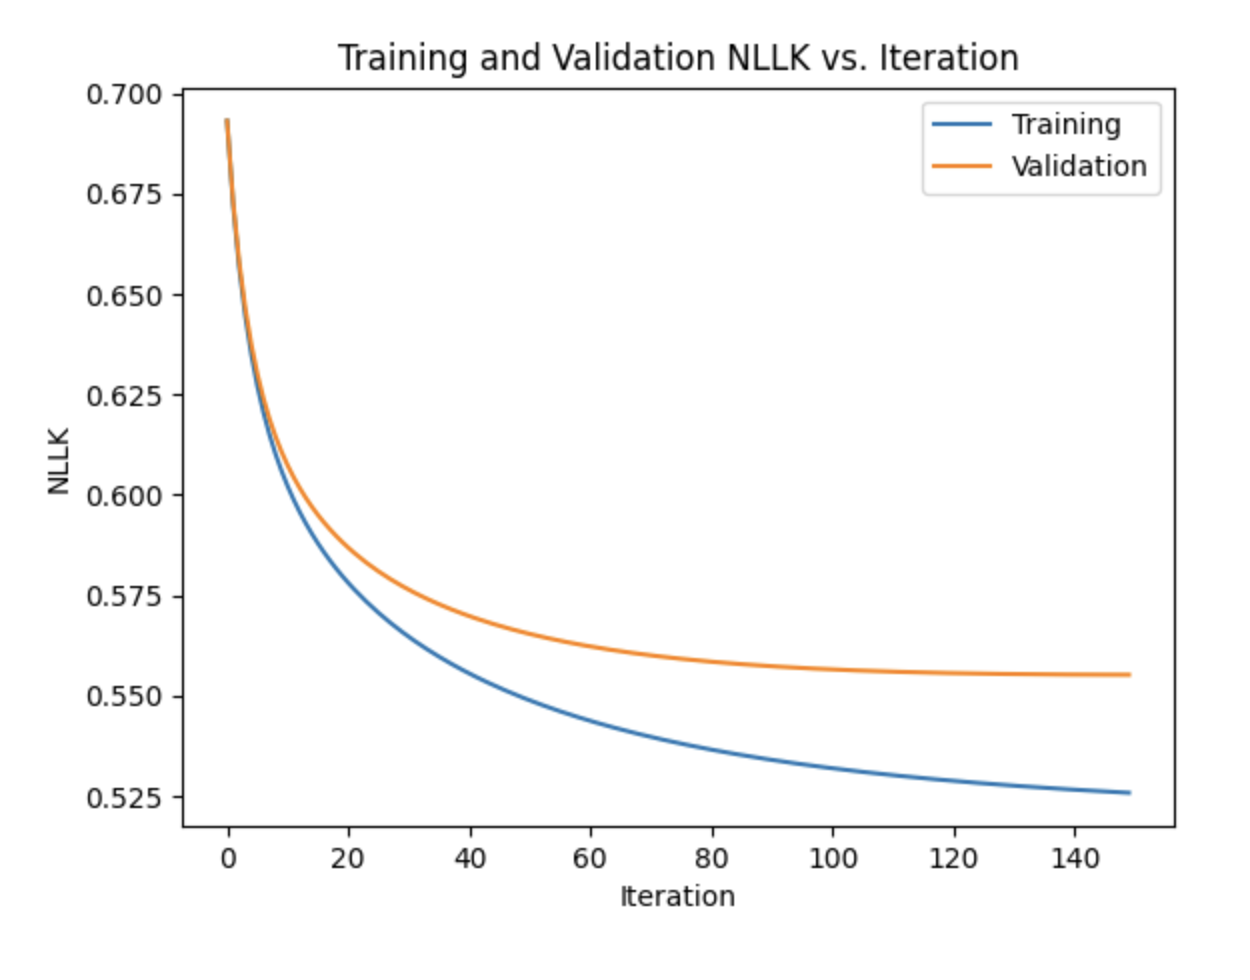
\includegraphics[width=0.8\textwidth]{q2b.png}
        \caption{Training and validation log likelihoods over 70 iterations, $lr =0.002$.}
        \label{fig:loss}
    \end{figure}

    \item The final validation and test accuracies with the reported hyperparameters are
    
    \begin{verbatim}
        validation accuracy = 0.7084391758396839
        test accuracy = 0.703076488851256
    \end{verbatim}

    \item With $j_1, j_2, j_3$ randomly sampled from the set of questions, the probabilities of a student with ability $\theta$ answering each question correctly are plotted below.
    
    \begin{figure}[H]
        \centering
        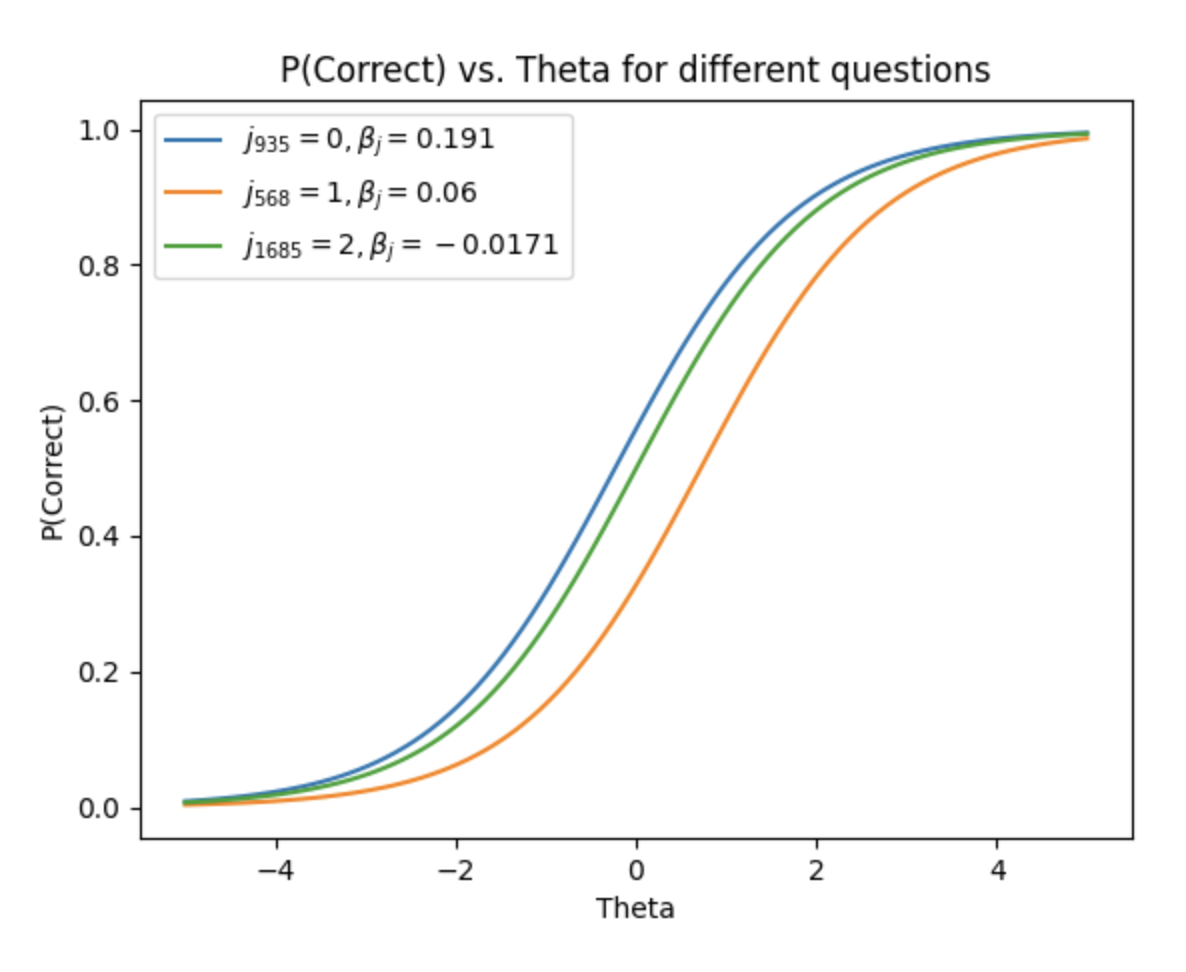
\includegraphics[width=0.8\textwidth]{q2d.png}
        \caption{Probabilities of a student with ability $\theta$ answering each question correctly.}
        \label{fig:probs}
    \end{figure}

    These curves are sigmoid-shaped, as expected -- they are the sigmoid function given by 

    \[\theta \mapsto \sigma(\theta - \beta_j)\]

    the curve for $j_{568}$, shifted the most to the right, corresponds to a higher value of $\beta_{568}$, indicating a question that is more difficult to answer correctly. The shape of the curves show that

    \[j_{935} < j_{1685} < j_{568}\]

    which suggests their difficulties are in the same order. We notice that as $\theta$ increases, the probabilities of answering each question correctly increase and approach $1$, becoming closer. This suggests that students with higher $\theta$ perceive all three questions to be similarly easy. 
    
    On the other hand, students with lower $\theta$ perceive the questions to be similarly difficult, with the question $j_{568}$ being the most difficult. It is students with $\theta$ close to $0$ that most clearly distinguish between the questions.
\end{enumerate}

\section{}

\begin{enumerate}[(a)]
    \item The function has been implemented in the files attached. Given $k \in \{1, 10, 50, 100, 200\}$, we found that $k^* = 10$ had the highest validation accuracy, and so we chose $k = 10$ as our final value. The validation and test accuracies are 
    
    \begin{verbatim}
        validation accuracy = 0.6586226361840248
        test accuracy = 0.6587637595258256
    \end{verbatim}

    \item A limitation of SVD is that we must fill in the missing entries in some fashion in order to apply a classical SVD algorithm. In our implementation, we choose to fill in missing values by taking the average on a per-question basis. This is a reasonable choice, but it is not clear that it is the best choice.
    
    There are other decisions that could be made, but this introduces an additional hyperparameter that is difficult to tune. 

    \item Implemented ALS with SGD in the code. 
    
    \item First, to tune the learning rate and number of iterations, we realized that $lr < 0.01$ resulted in slow convergence, whereas $lr \geq 0.1$ resulted in non-monotonic convergence. Thus, $lr = 0.05$ was chosen. It was also observed that $100000$ iterations was sufficient for convergence while still maintaining a reasonable runtime.
    
    For $k \in \{1, 10, 50, 70, 100, 200\}$, we found that $k^* = 70$ had the highest validation accuracy, and so we chose $k = 70$ as our final value. 
    \item Here is a plot of training and validation squared error over 100000 iterations, with $lr = 0.05$ and $k = 70$. We consider average squared error loss taken over the training and validation datasets. 
    
    \begin{figure}[H]
        \centering
        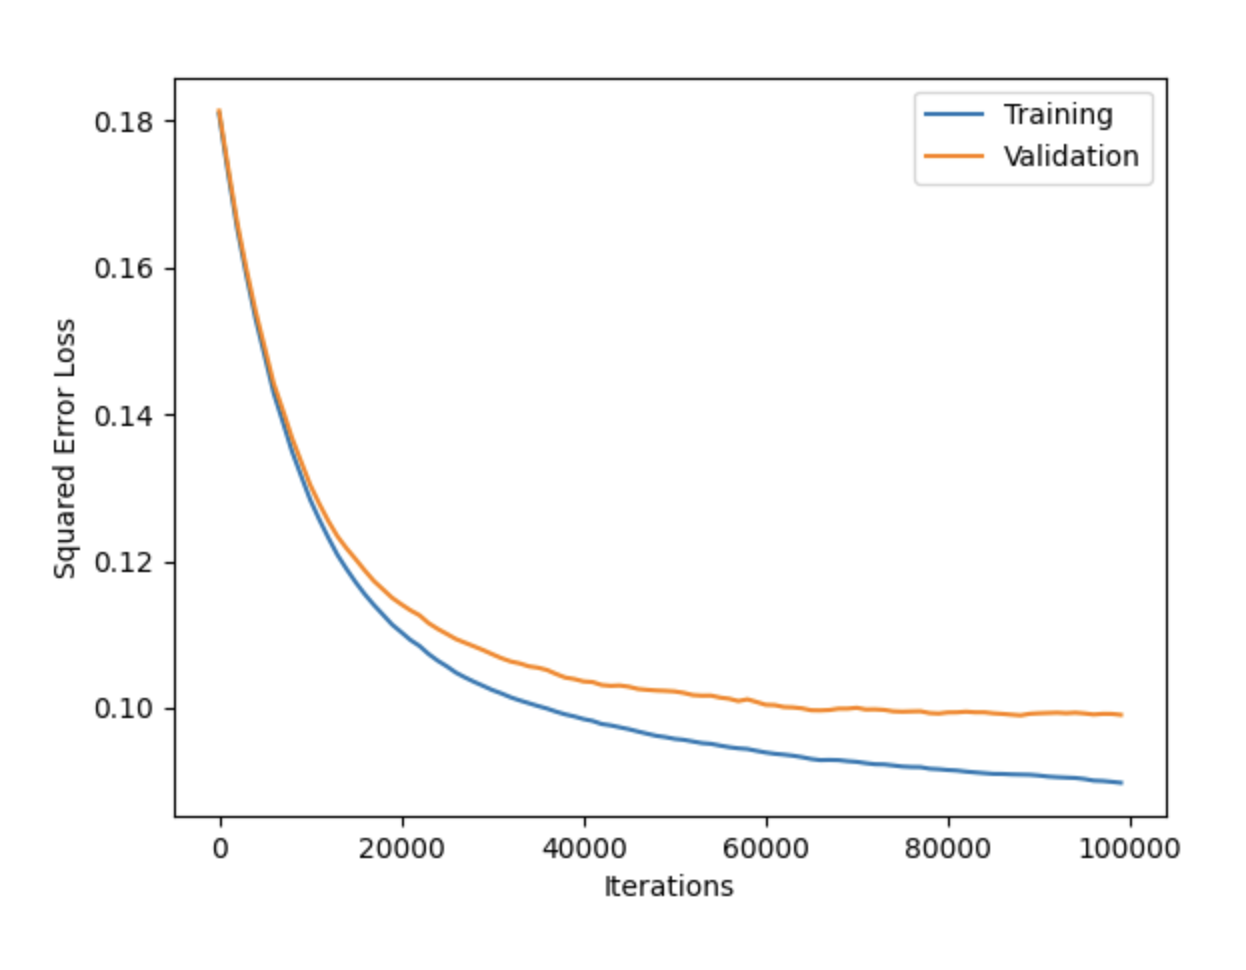
\includegraphics[width=0.8\textwidth]{q3e.png}
        \caption{Training and validation squared error over 100000 iterations, $lr = 0.05$, $k = 70$.}
        \label{fig:loss}
    \end{figure}

    We see that both training and validation losses decrease monotonically, with validation loss approaching a plateau after $100000$ iterations. This suggests that the model is not overfitting, and that the model has converged.
    
    
    The final validation and test accuracies are

    \begin{verbatim}
        Validation: 0.6972904318374259
        Test: 0.6948913350268134
    \end{verbatim}

\end{enumerate}

\end{document}
